\documentclass[border=8pt]{standalone}
\usepackage[T1]{fontenc}\usepackage{helvet}\renewcommand{\familydefault}{\sfdefault}
\usepackage{tikz}\usetikzlibrary{arrows.meta, positioning, calc, backgrounds}
\definecolor{ink}{HTML}{1a1916}
\definecolor{inktwo}{HTML}{3a3a35}
\definecolor{inkthree}{HTML}{6a6862}
\definecolor{rule}{HTML}{b8b09a}
\definecolor{amber}{HTML}{a8730a}
\definecolor{red}{HTML}{c8261a}
\definecolor{paper}{HTML}{f0eee5}
\definecolor{slab}{HTML}{d8d4c6}
\tikzset{
  >={Stealth[length=2.2mm]},
  wire/.style={line width=0.8pt, ink},
  modwire/.style={line width=0.6pt, dashed, ink},
  tastewire/.style={line width=0.6pt, dashed, amber},
  gatewire/.style={line width=0.6pt, dotted, ink},
  block/.style={rectangle, draw=ink, line width=0.9pt, fill=slab, minimum width=3.0cm, minimum height=1.9cm, inner sep=0pt},
  perf/.style={rectangle, draw=ink, line width=0.7pt, minimum width=3.0cm, minimum height=0.7cm, inner sep=2pt, font=\footnotesize, text=ink},
  title/.style={font=\scriptsize\bfseries, text=ink, anchor=north, inner sep=2pt},
  jack/.style={circle, draw=ink, fill=paper, line width=0.5pt, minimum size=3.2pt, inner sep=0pt},
  plabel/.style={font=\tiny, text=inktwo, anchor=west, inner sep=1pt},
  olabel/.style={font=\tiny, text=inktwo, anchor=east, inner sep=1pt},
  settings/.style={font=\scriptsize, text=ink, align=left, anchor=north west, inner sep=1pt, text width=2.9cm},
}
\begin{document}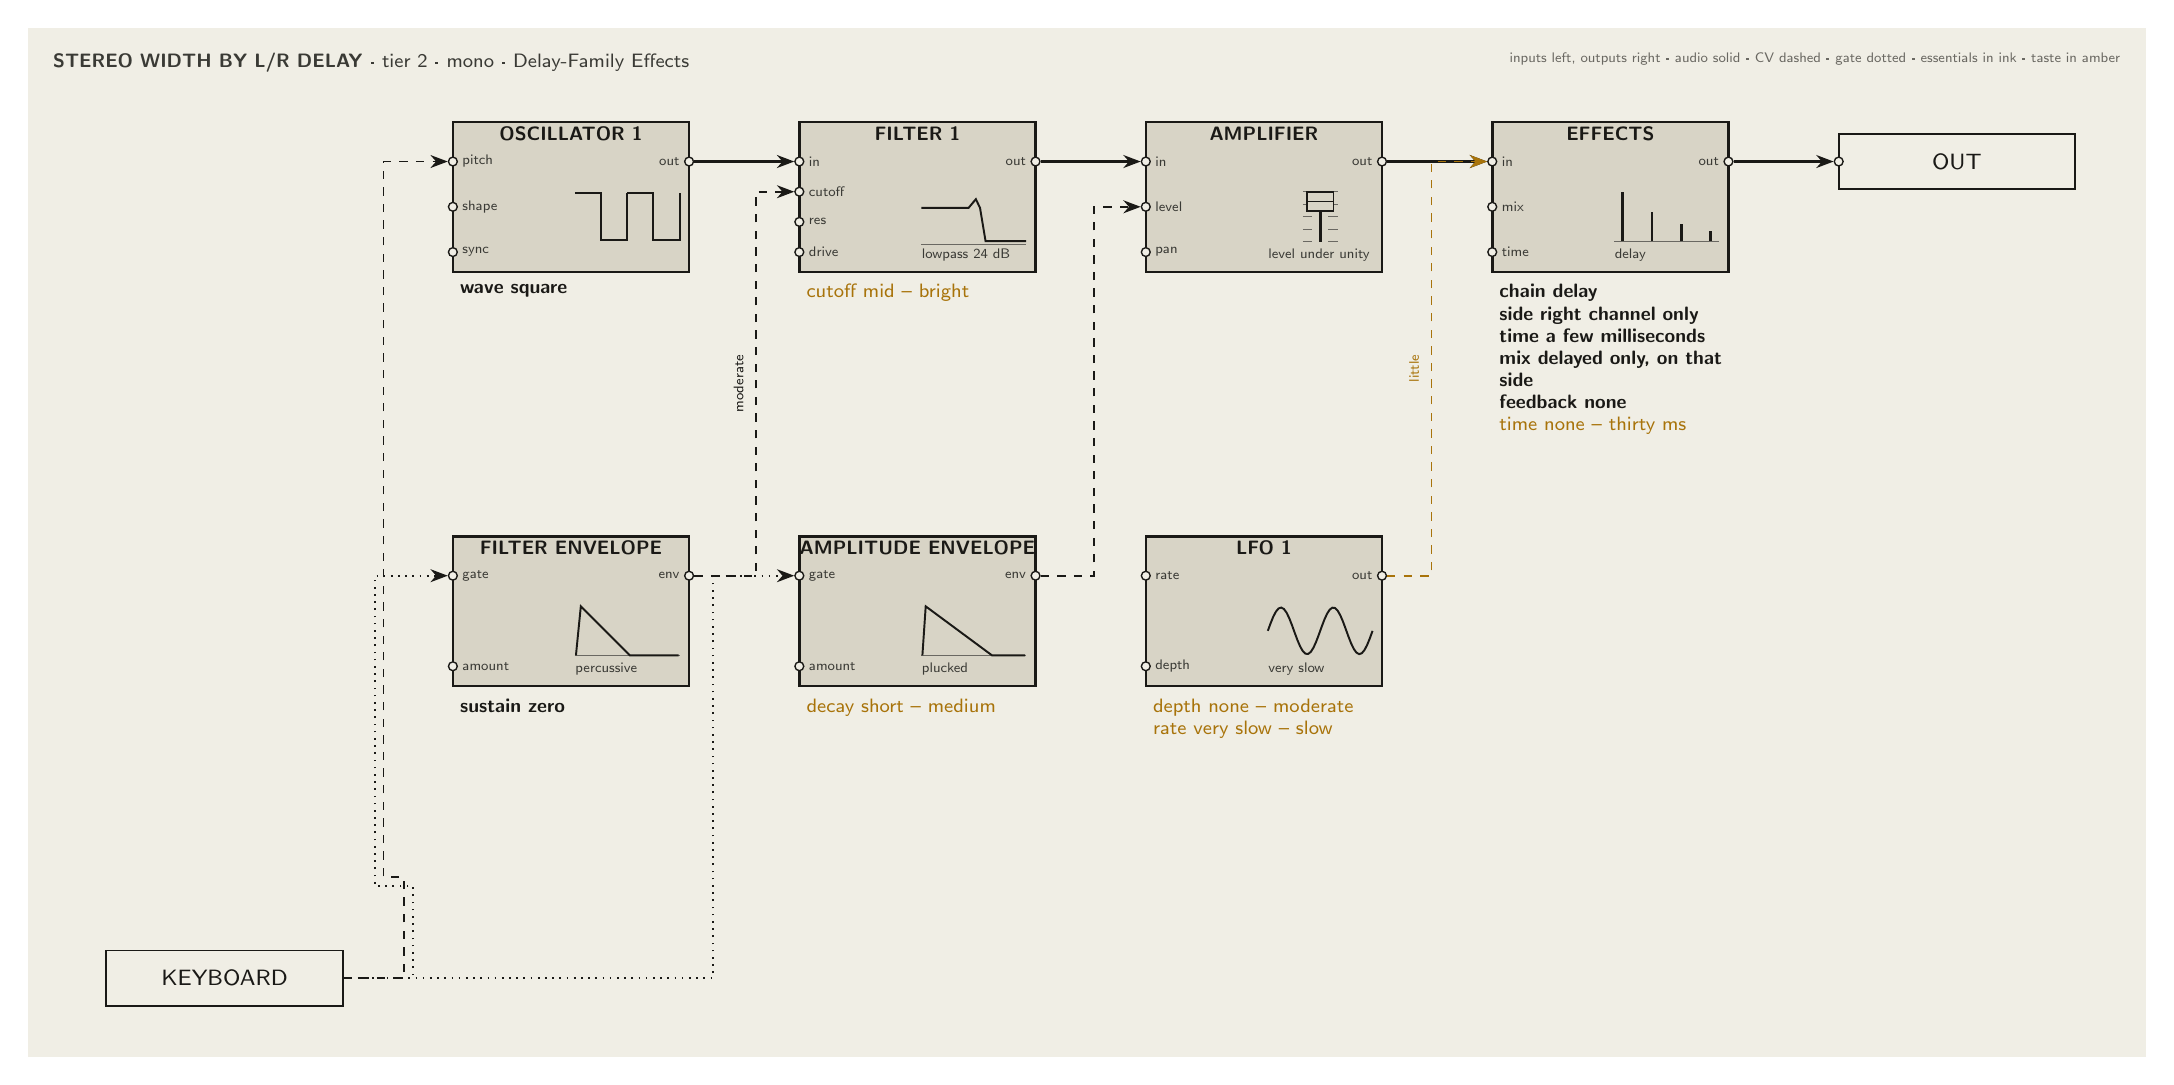
\begin{tikzpicture}
\begin{scope}[on background layer]\fill[paper] (-2.5,-10.92) rectangle (24.4,2.15);\end{scope}
\node[block, minimum height=1.9cm] (osc1) at (4.4,0.0) {};
\node[title] at (osc1.north) {OSCILLATOR 1};
\node[jack] (osc1-pitch) at (2.9000000000000004,0.44999999999999996) {};
\node[plabel] at (2.9800000000000004,0.44999999999999996) {pitch};
\node[jack] (osc1-shape) at (2.9000000000000004,-0.125) {};
\node[plabel] at (2.9800000000000004,-0.125) {shape};
\node[jack] (osc1-sync) at (2.9000000000000004,-0.7) {};
\node[plabel] at (2.9800000000000004,-0.7) {sync};
\node[jack] (osc1-out) at (5.9,0.44999999999999996) {};
\node[olabel] at (5.82,0.44999999999999996) {out};
\begin{scope}
\draw[ink, line width=0.7pt] (4.450,0.046) -- (4.783,0.046) -- (4.783,-0.546) -- (5.115,-0.546) -- (5.115,0.046);
\draw[ink, line width=0.7pt] (5.115,0.046) -- (5.447,0.046) -- (5.447,-0.546) -- (5.780,-0.546) -- (5.780,0.046);
\end{scope}
\node[settings] at (2.95,-1.0699999999999998) {\textbf{wave square}};
\node[block, minimum height=1.9cm] (filter1) at (8.8,0.0) {};
\node[title] at (filter1.north) {FILTER 1};
\node[jack] (filter1-in) at (7.300000000000001,0.44999999999999996) {};
\node[plabel] at (7.380000000000001,0.44999999999999996) {in};
\node[jack] (filter1-cutoff) at (7.300000000000001,0.06666666666666665) {};
\node[plabel] at (7.380000000000001,0.06666666666666665) {cutoff};
\node[jack] (filter1-res) at (7.300000000000001,-0.31666666666666665) {};
\node[plabel] at (7.380000000000001,-0.31666666666666665) {res};
\node[jack] (filter1-drive) at (7.300000000000001,-0.7) {};
\node[plabel] at (7.380000000000001,-0.7) {drive};
\node[jack] (filter1-out) at (10.3,0.44999999999999996) {};
\node[olabel] at (10.22,0.44999999999999996) {out};
\begin{scope}
\draw[inkthree, line width=0.3pt] (8.850,-0.605) -- (10.180,-0.605);
\draw[ink, line width=0.7pt] (8.850,-0.139) -- (9.449,-0.139) -- (9.542,-0.028) -- (9.595,-0.139) -- (9.665,-0.561) -- (10.180,-0.561);
\node[font=\tiny, text=inktwo, anchor=north west, inner sep=0pt] at (8.850,-0.650) {lowpass 24 dB};
\end{scope}
\node[settings] at (7.3500000000000005,-1.0699999999999998) {\textcolor{amber}{cutoff mid -- bright}};
\node[block, minimum height=1.9cm] (amp) at (13.200000000000001,0.0) {};
\node[title] at (amp.north) {AMPLIFIER};
\node[jack] (amp-in) at (11.700000000000001,0.44999999999999996) {};
\node[plabel] at (11.780000000000001,0.44999999999999996) {in};
\node[jack] (amp-level) at (11.700000000000001,-0.125) {};
\node[plabel] at (11.780000000000001,-0.125) {level};
\node[jack] (amp-pan) at (11.700000000000001,-0.7) {};
\node[plabel] at (11.780000000000001,-0.7) {pan};
\node[jack] (amp-out) at (14.700000000000001,0.44999999999999996) {};
\node[olabel] at (14.620000000000001,0.44999999999999996) {out};
\begin{scope}
\draw[ink, line width=1.2pt] (13.915,-0.570) -- (13.915,0.070);
\draw[inkthree, line width=0.3pt] (13.695,-0.570) -- (13.815,-0.570) (14.015,-0.570) -- (14.135,-0.570);
\draw[inkthree, line width=0.3pt] (13.695,-0.410) -- (13.815,-0.410) (14.015,-0.410) -- (14.135,-0.410);
\draw[inkthree, line width=0.3pt] (13.695,-0.250) -- (13.815,-0.250) (14.015,-0.250) -- (14.135,-0.250);
\draw[inkthree, line width=0.3pt] (13.695,-0.090) -- (13.815,-0.090) (14.015,-0.090) -- (14.135,-0.090);
\draw[inkthree, line width=0.3pt] (13.695,0.070) -- (13.815,0.070) (14.015,0.070) -- (14.135,0.070);
\fill[slab, draw=ink, line width=0.6pt] (13.745,-0.178) rectangle (14.085,0.062);
\draw[ink, line width=0.5pt] (13.745,-0.058) -- (14.085,-0.058);
\node[font=\tiny, text=inktwo, anchor=north west, inner sep=0pt] at (13.250,-0.650) {level under unity};
\end{scope}
\node[block, minimum height=1.9cm] (fx) at (17.6,0.0) {};
\node[title] at (fx.north) {EFFECTS};
\node[jack] (fx-in) at (16.1,0.44999999999999996) {};
\node[plabel] at (16.18,0.44999999999999996) {in};
\node[jack] (fx-mix) at (16.1,-0.125) {};
\node[plabel] at (16.18,-0.125) {mix};
\node[jack] (fx-time) at (16.1,-0.7) {};
\node[plabel] at (16.18,-0.7) {time};
\node[jack] (fx-out) at (19.1,0.44999999999999996) {};
\node[olabel] at (19.020000000000003,0.44999999999999996) {out};
\begin{scope}
\draw[inkthree, line width=0.3pt] (17.650,-0.561) -- (18.980,-0.561);
\draw[ink, line width=0.9pt] (17.756,-0.561) -- (17.756,0.061);
\draw[ink, line width=0.9pt] (18.129,-0.561) -- (18.129,-0.188);
\draw[ink, line width=0.9pt] (18.501,-0.561) -- (18.501,-0.337);
\draw[ink, line width=0.9pt] (18.874,-0.561) -- (18.874,-0.427);
\node[font=\tiny, text=inktwo, anchor=north west, inner sep=0pt] at (17.650,-0.650) {delay};
\end{scope}
\node[settings] at (16.150000000000002,-1.0699999999999998) {\textbf{chain delay} \\ \textbf{side right channel only} \\ \textbf{time a few milliseconds} \\ \textbf{mix delayed only, on that side} \\ \textbf{feedback none} \\ \textcolor{amber}{time none -- thirty ms}};
\node[block, minimum height=1.9cm] (fenv) at (4.4,-5.26) {};
\node[title] at (fenv.north) {FILTER ENVELOPE};
\node[jack] (fenv-gate) at (2.9000000000000004,-4.81) {};
\node[plabel] at (2.9800000000000004,-4.81) {gate};
\node[jack] (fenv-amount) at (2.9000000000000004,-5.959999999999999) {};
\node[plabel] at (2.9800000000000004,-5.959999999999999) {amount};
\node[jack] (fenv-out) at (5.9,-4.81) {};
\node[olabel] at (5.82,-4.81) {env};
\begin{scope}
\draw[inkthree, line width=0.3pt] (4.450,-5.821) -- (5.780,-5.821);
\draw[ink, line width=0.7pt] (4.463,-5.821) -- (4.525,-5.199) -- (5.146,-5.821) -- (5.146,-5.821) -- (5.767,-5.821);
\node[font=\tiny, text=inktwo, anchor=north west, inner sep=0pt] at (4.450,-5.910) {percussive};
\end{scope}
\node[settings] at (2.95,-6.33) {\textbf{sustain zero}};
\node[block, minimum height=1.9cm] (aenv) at (8.8,-5.26) {};
\node[title] at (aenv.north) {AMPLITUDE ENVELOPE};
\node[jack] (aenv-gate) at (7.300000000000001,-4.81) {};
\node[plabel] at (7.380000000000001,-4.81) {gate};
\node[jack] (aenv-amount) at (7.300000000000001,-5.959999999999999) {};
\node[plabel] at (7.380000000000001,-5.959999999999999) {amount};
\node[jack] (aenv-out) at (10.3,-4.81) {};
\node[olabel] at (10.22,-4.81) {env};
\begin{scope}
\draw[inkthree, line width=0.3pt] (8.850,-5.821) -- (10.180,-5.821);
\draw[ink, line width=0.7pt] (8.863,-5.821) -- (8.905,-5.199) -- (9.746,-5.821) -- (9.746,-5.821) -- (10.167,-5.821);
\node[font=\tiny, text=inktwo, anchor=north west, inner sep=0pt] at (8.850,-5.910) {plucked};
\end{scope}
\node[settings] at (7.3500000000000005,-6.33) {\textcolor{amber}{decay short -- medium}};
\node[block, minimum height=1.9cm] (lfo1) at (13.200000000000001,-5.26) {};
\node[title] at (lfo1.north) {LFO 1};
\node[jack] (lfo1-rate) at (11.700000000000001,-4.81) {};
\node[plabel] at (11.780000000000001,-4.81) {rate};
\node[jack] (lfo1-depth) at (11.700000000000001,-5.959999999999999) {};
\node[plabel] at (11.780000000000001,-5.959999999999999) {depth};
\node[jack] (lfo1-out) at (14.700000000000001,-4.81) {};
\node[olabel] at (14.620000000000001,-4.81) {out};
\begin{scope}
\draw[ink, line width=0.7pt] plot[domain=0:1, samples=40, variable=\u] ({13.250+\u*1.330},{-5.880+(0.740)*(0.5+0.4*sin(360*\u*2))});
\node[font=\tiny, text=inktwo, anchor=north west, inner sep=0pt] at (13.250,-5.910) {very slow};
\end{scope}
\node[settings] at (11.750000000000002,-6.33) {\textcolor{amber}{depth none -- moderate} \\ \textcolor{amber}{rate very slow -- slow}};
\node[perf] (key) at (0.0,-9.92) {KEYBOARD};
\node[perf, fill=paper] (out) at (22.0,0.44999999999999996) {OUT}; \node[jack] (out-in) at (20.5,0.44999999999999996) {};
\draw[wire,->] (osc1-out) -- (filter1-in);
\draw[wire,->] (filter1-out) -- (amp-in);
\draw[wire,->] (amp-out) -- (fx-in);
\draw[wire,->] (fx-out) -- (out-in);
\draw[modwire,->] (fenv-out) -- (6.750000000000001,-4.81) -- (6.750000000000001,0.06666666666666665) -- (filter1-cutoff);
\node[font=\tiny, text=ink, anchor=south, inner sep=1pt, rotate=90] at (6.630000000000001,-2.3716666666666666) {moderate};
\draw[modwire,->] (aenv-out) -- (11.040000000000001,-4.81) -- (11.040000000000001,-0.125) -- (amp-level);
\draw[tastewire,->] (lfo1-out) -- (15.33,-4.81) -- (15.33,0.44999999999999996) -- (fx-in);
\node[font=\tiny, text=amber, anchor=south, inner sep=1pt, rotate=90] at (15.21,-2.1799999999999997) {little};
\draw[modwire,->] (key.east) -- (2.28,-9.92) -- (2.28,-8.64) -- (2.0200000000000005,-8.64) -- (2.0200000000000005,0.44999999999999996) -- (osc1-pitch);
\draw[gatewire,->] (key.east) -- (2.39,-9.92) -- (2.39,-8.75) -- (1.9100000000000006,-8.75) -- (1.9100000000000006,-4.81) -- (fenv-gate);
\draw[gatewire,->] (key.east) -- (6.200000000000001,-9.92) -- (6.200000000000001,-4.81) -- (aenv-gate);
\node[anchor=north west, font=\scriptsize, text=inktwo] at (-2.3,1.95) {\textbf{STEREO WIDTH BY L/R DELAY} · tier 2 · mono · Delay-Family Effects};
\node[anchor=north east, font=\tiny, text=inkthree] at (24.2,1.95) {inputs left, outputs right · audio solid · CV dashed · gate dotted · essentials in ink · taste in amber};
\end{tikzpicture}\end{document}
